%==============================================================================
%== template for LATEX poster =================================================
%==============================================================================
%
%--A0 beamer slide-------------------------------------------------------------
\documentclass[final]{beamer}\usepackage[]{graphicx}\usepackage[]{color}
%% maxwidth is the original width if it is less than linewidth
%% otherwise use linewidth (to make sure the graphics do not exceed the margin)
\makeatletter
\def\maxwidth{ %
  \ifdim\Gin@nat@width>\linewidth
    \linewidth
  \else
    \Gin@nat@width
  \fi
}
\makeatother

\definecolor{fgcolor}{rgb}{0.345, 0.345, 0.345}
\newcommand{\hlnum}[1]{\textcolor[rgb]{0.686,0.059,0.569}{#1}}%
\newcommand{\hlstr}[1]{\textcolor[rgb]{0.192,0.494,0.8}{#1}}%
\newcommand{\hlcom}[1]{\textcolor[rgb]{0.678,0.584,0.686}{\textit{#1}}}%
\newcommand{\hlopt}[1]{\textcolor[rgb]{0,0,0}{#1}}%
\newcommand{\hlstd}[1]{\textcolor[rgb]{0.345,0.345,0.345}{#1}}%
\newcommand{\hlkwa}[1]{\textcolor[rgb]{0.161,0.373,0.58}{\textbf{#1}}}%
\newcommand{\hlkwb}[1]{\textcolor[rgb]{0.69,0.353,0.396}{#1}}%
\newcommand{\hlkwc}[1]{\textcolor[rgb]{0.333,0.667,0.333}{#1}}%
\newcommand{\hlkwd}[1]{\textcolor[rgb]{0.737,0.353,0.396}{\textbf{#1}}}%

\usepackage{framed}
\makeatletter
\newenvironment{kframe}{%
 \def\at@end@of@kframe{}%
 \ifinner\ifhmode%
  \def\at@end@of@kframe{\end{minipage}}%
  \begin{minipage}{\columnwidth}%
 \fi\fi%
 \def\FrameCommand##1{\hskip\@totalleftmargin \hskip-\fboxsep
 \colorbox{shadecolor}{##1}\hskip-\fboxsep
     % There is no \\@totalrightmargin, so:
     \hskip-\linewidth \hskip-\@totalleftmargin \hskip\columnwidth}%
 \MakeFramed {\advance\hsize-\width
   \@totalleftmargin\z@ \linewidth\hsize
   \@setminipage}}%
 {\par\unskip\endMakeFramed%
 \at@end@of@kframe}
\makeatother

\definecolor{shadecolor}{rgb}{.97, .97, .97}
\definecolor{messagecolor}{rgb}{0, 0, 0}
\definecolor{warningcolor}{rgb}{1, 0, 1}
\definecolor{errorcolor}{rgb}{1, 0, 0}
\newenvironment{knitrout}{}{} % an empty environment to be redefined in TeX

\usepackage{alltt}
\usepackage{graphicx, color}
%% maxwidth is the original width if it is less than linewidth
%% otherwise use linewidth (to make sure the graphics do not exceed the margin)
\makeatletter
\def\maxwidth{ %
  \ifdim\Gin@nat@width>\linewidth
    \linewidth
  \else
    \Gin@nat@width
  \fi
}
\makeatother

\usepackage[
  natbib = true,
    backend=bibtex,
    isbn=false,
    url=false,
    doi=false,
    eprint=false,
]{biblatex}
%{\tiny
\bibliography{CT_Skull_Stripping}
%}
\renewcommand*{\bibfont}{\scriptsize}

\usepackage{array}

%\graphicspath{{../maps/}{../}}


\def\newblock{\hskip .11em plus .33em minus .07em} %for natbib and beamer 
\usepackage[orientation=landscape,size=a0,
            scale=1,         % font scale factor
            size=custom,width=140,height=83,
           ]{beamerposter}
\setbeamertemplate{frametitle}{
    \vspace{-5cm}\\
    \insertframetitle
}         
           
\geometry{
  hmargin=2.5cm, % little modification of margins
  vmargin = 0cm,
  head=0cm  
}

\usepackage{multirow}
%
%\usepackage{float}
%\usepackage{subfigure}

%\usepackage{caption}
%\captionsetup{compatibility=false}
%\usepackage{subcaption}

%\usepackage{sidecap}

\usepackage{subfig}

\usepackage{tikz}
\usetikzlibrary{shapes,arrows}
\usetikzlibrary{positioning}

\usepackage{adjustbox}

\usepackage[utf8]{inputenc}
%\usepackage{verbatim}

\linespread{1.15}
%
%==The poster style============================================================
\usetheme{sharelatex}

%==Title, date and authors of the poster=======================================
\title
%[Super Conference, 1 - 10 July 2013, New York, USA] % Conference
{ % Poster title
Validated Automatic Brain Extraction of Head CT Images
}




\author{ % Authors
John Muschelli$^{1}$, Natalie~L.~Ullman$^{2}$, Paul~Vespa$^{3}$, Daniel F. Hanley$^{2}$, Ciprian~M.~Crainiceanu$^{1}$
}

%
%\cortext[cor1]{Principal Corresponding Author}
%\address[jhsph]{Department of Biostatistics, Bloomberg School of Public Health, Johns Hopkins University, Baltimore, MD, USA}
%\address[jhmi]{Department of Neurology, Division of Brain Injury Outcomes,  Johns Hopkins Medical Institutions, Baltimore, MD, USA}
%\address[ucla]{Department of Neurosurgery, David Geffen School of Medicine at UCLA, Los Angeles, CA, USA}



\institute
[Johns Hopkins Bloomberg School of Public Health] % General University
{
%Johns Hopkins Bloomberg School of Public Health
\bf{1} Department of Biostatistics, Bloomberg School of Public Health, Johns Hopkins University, Baltimore, MD, USA \\
\bf{2} Department of Neurology, Division of Brain Injury Outcomes,  Johns Hopkins Medical Institutions, Baltimore, MD, USA\\
\bf{3} Department of Neurosurgery, David Geffen School of Medicine at UCLA, Los Angeles, CA, USA
}
\date{\today}


\usepackage{hyperref}
\IfFileExists{upquote.sty}{\usepackage{upquote}}{}
\begin{document}

\vspace{-4cm}
\newcommand{\stickynote}{\includegraphics[height=1.5em]{blank_sticky_note.png}\;}
\renewcommand{\thesubfigure}{\Alph{subfigure}}


\begin{frame}[fragile]
\vspace{-4cm}












%==============================================================================
%\begin{multicols}{2}
\begin{minipage}{0.2\linewidth}
\section{Image Processing Pipeline}
\includegraphics[width=\linewidth]{Imaging_Pipeline_Flowchart.pdf}
\section{Sources of Funding}
{\scriptsize
The project described and data used were supported by the NIH grants RO1EB012547, T32AG000247, R01NS046309, RO1NS060910, RO1NS085211, R01NS046309, U01NS080824, U01NS080824 and U01NS062851 and RO1MH095836.
}
\end{minipage}
\begin{minipage}{0.39\linewidth}







%==============================================================================
%==The poster content==========================================================
%==============================================================================
\section{Goals and Methods}
\begin{multicols}{2}
Systematically analyze the performance of the brain extraction tool (BET) \citep{smith_fast_2002}, a function of the FMRIB software library (FSL) \citep{jenkinson_fsl_2012}, on head CT images of patients with intracranial hemorrhage by varying parameters of BET and the use of smoothing after performing CT-specific preprocessing by:
\begin{itemize}
\item Quantitatively comparing the results to the manual gold standard, and
\item Estimating the performance using the intraclass correlation of serial CT scans.
\end{itemize}


\vfill
\columnbreak


%\section{Methods}


Data were from patients with intracranial hemorrhage from MISTIE (Minimally Invasive Surgery plus recombinant-tissue plasminogen activator for Intracerebral Evacuation) stroke trial centers.
\begin{itemize}
\item Sample compared to gold standard: Thirty Six images from 36 patients. 
\item Intraclass Correlation Estimate: 1062 images from 133 patients, after excluding 115 scans for craniotomy or skull stripping failure (9.8\%).  
\end{itemize}
\end{multicols}
%
%\begin{figure}
%\centering
%\begin{tabular}{m{0.3\linewidth}>{\centering}m{0.3\linewidth}p{0.2\linewidth}}
%Data were from patients with intracranial hemorrhage from MISTIE (Minimally Invasive Surgery plus recombinant-tissue plasminogen activator for Intracerebral Evacuation) stroke trial centers.
%\begin{itemize}
%\item Sample compared to gold standard: num_scans images from npt patients. 
%\item Intraclass Correlation Estimate: num_scans.icc images from npt.icc patients, after excluding fail scans for craniotomy or skull stripping failure (pct.fail\%).  
%\end{itemize} &
%\includegraphics[scale=0.7]{Imaging_Pipeline_Flowchart.pdf} & 
%\multirow{1}{\linewidth}[5\baselineskip]{{\bf Figure: Processing Pipeline.} Each image was thresholded using a $0-100$ Hounsfield units (HU) range. In one variant of the pipeline, data were smoothed using a Gaussian kernel ($\sigma=1$mm) and re-thresholded to $0$-$100$ HU; in the other, data were not smoothed.  BET was applied using 1 of 3 fractional intensity (FI) thresholds: $0.01$, $0.1$, $0.35$ and holes in the brain mask produced by BET were filled. }
%\end{tabular}
%\end{figure}



\section{Measuring and Testing Brain Extraction Performance}








\begin{tabular}{cc}
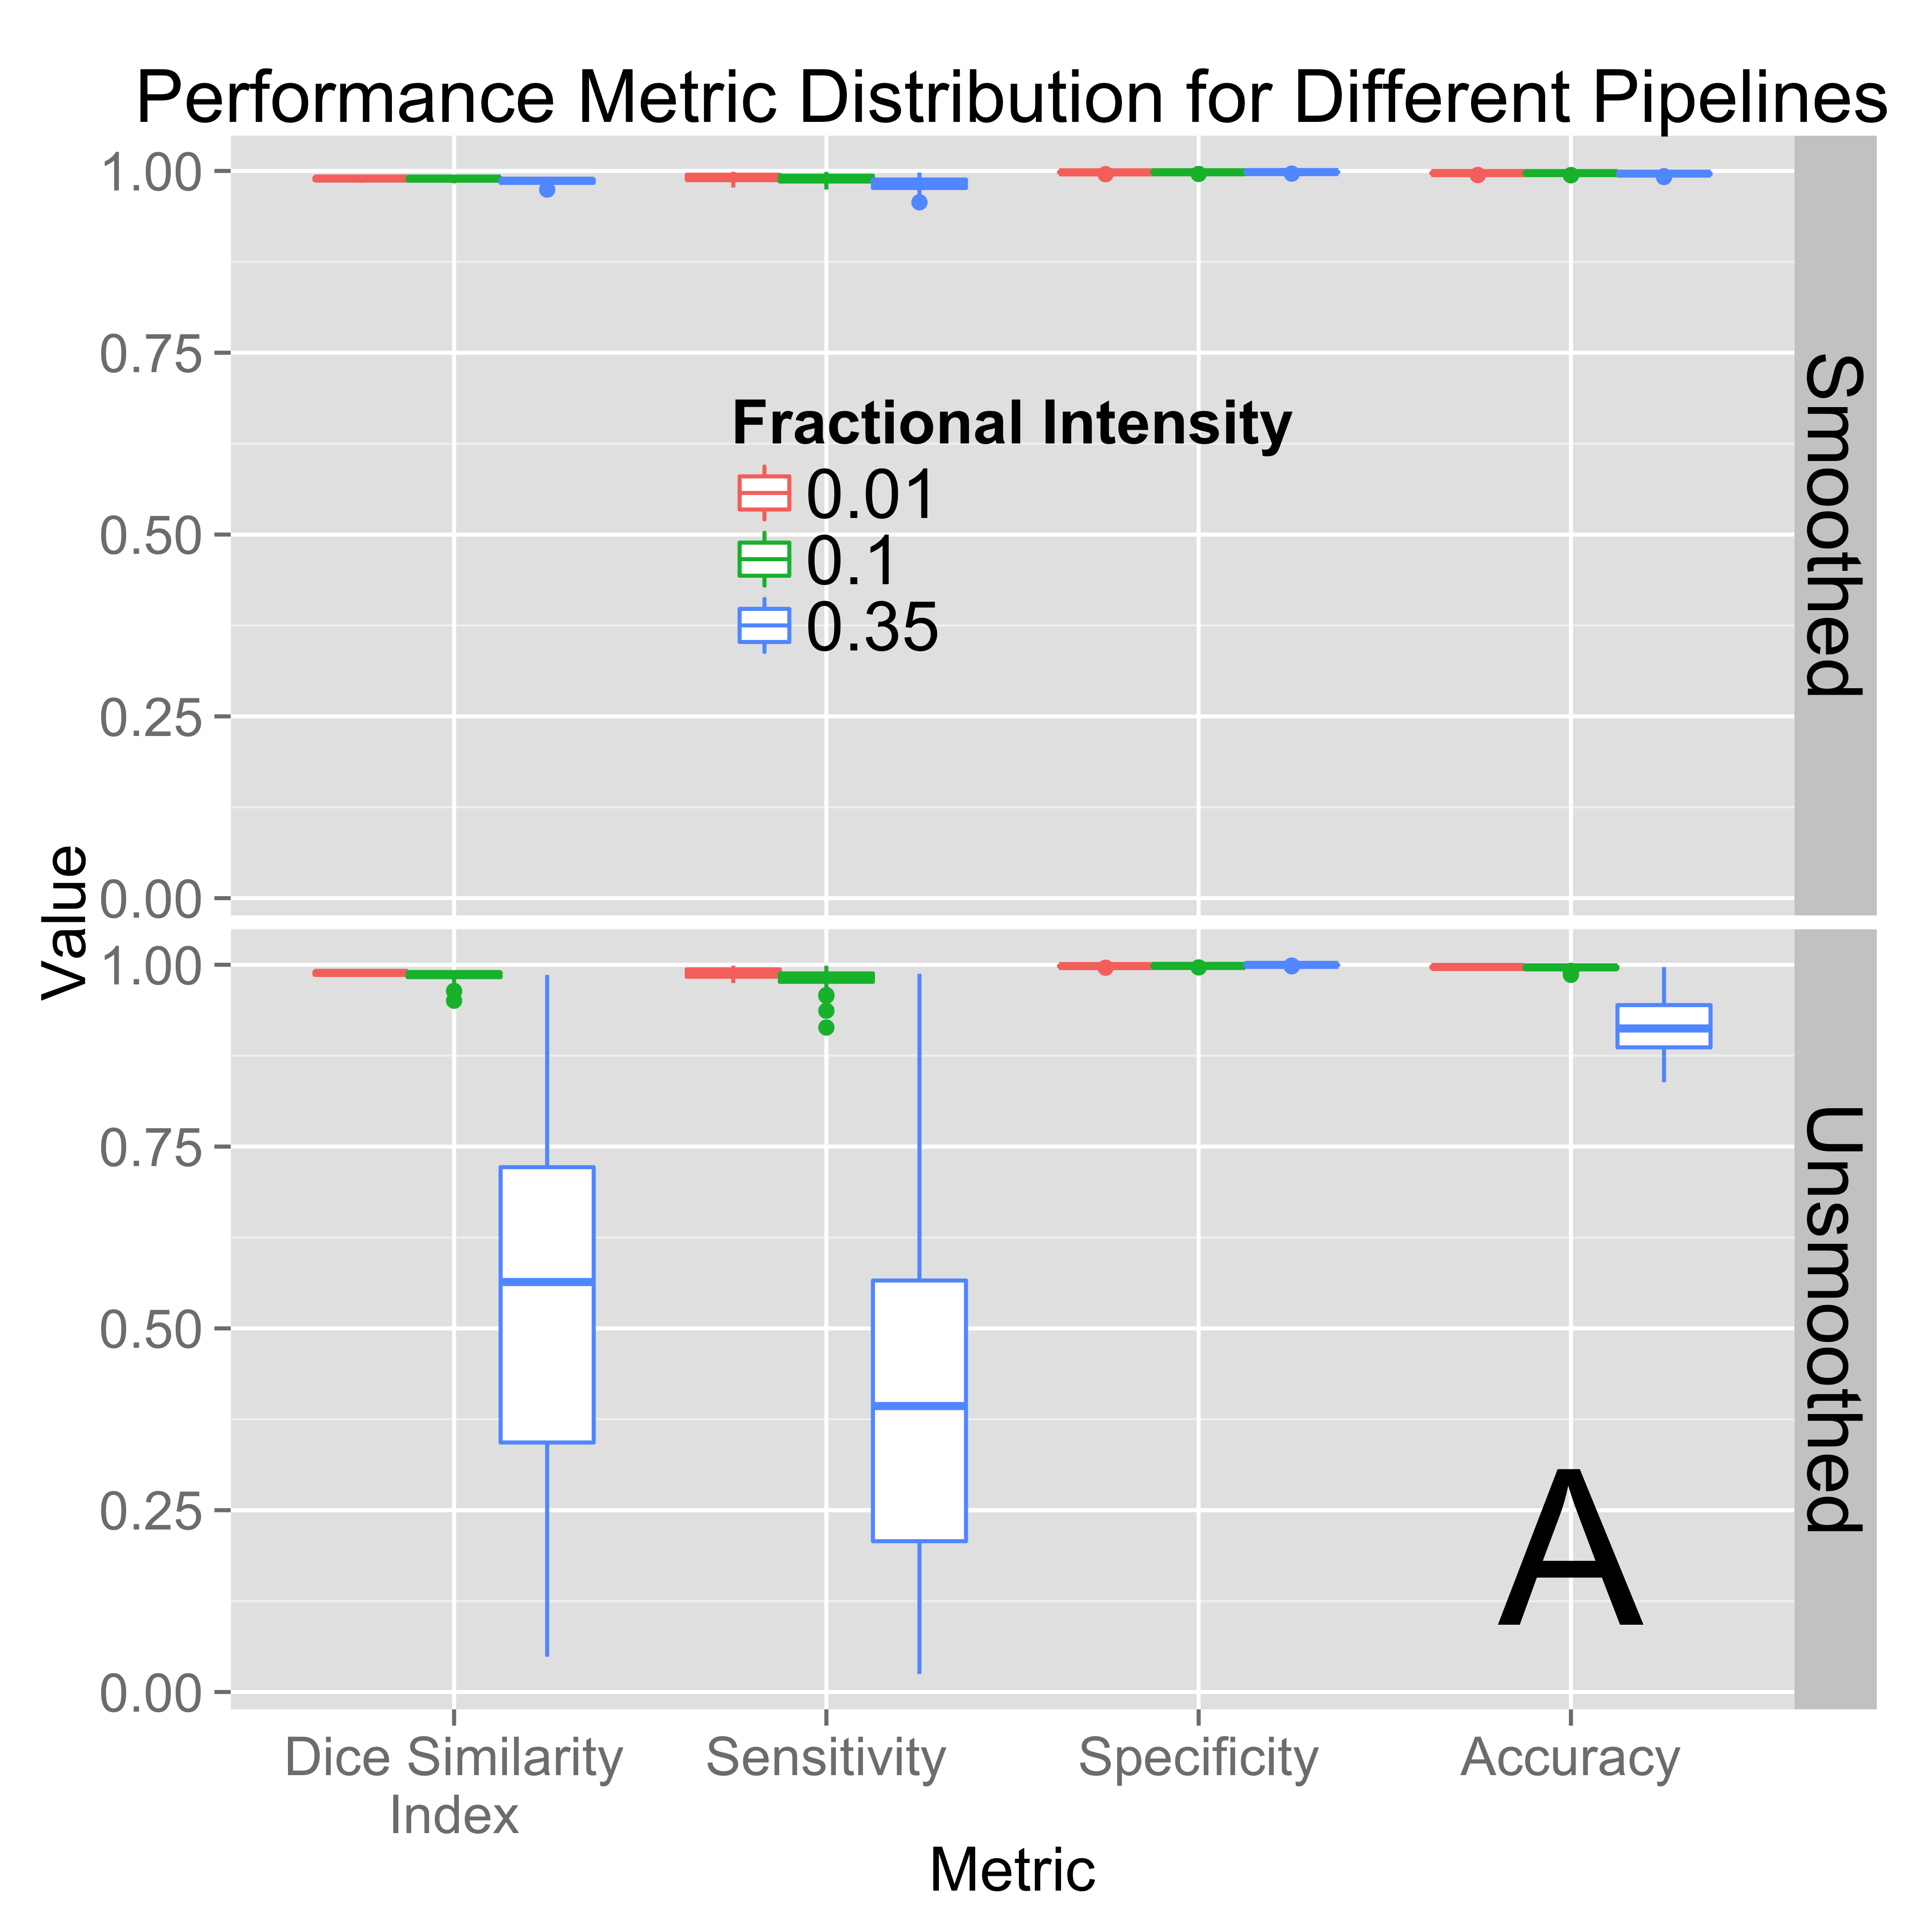
\includegraphics[width=0.46\linewidth]{figure/CT_Skull_Stripping_Figure2.png} &
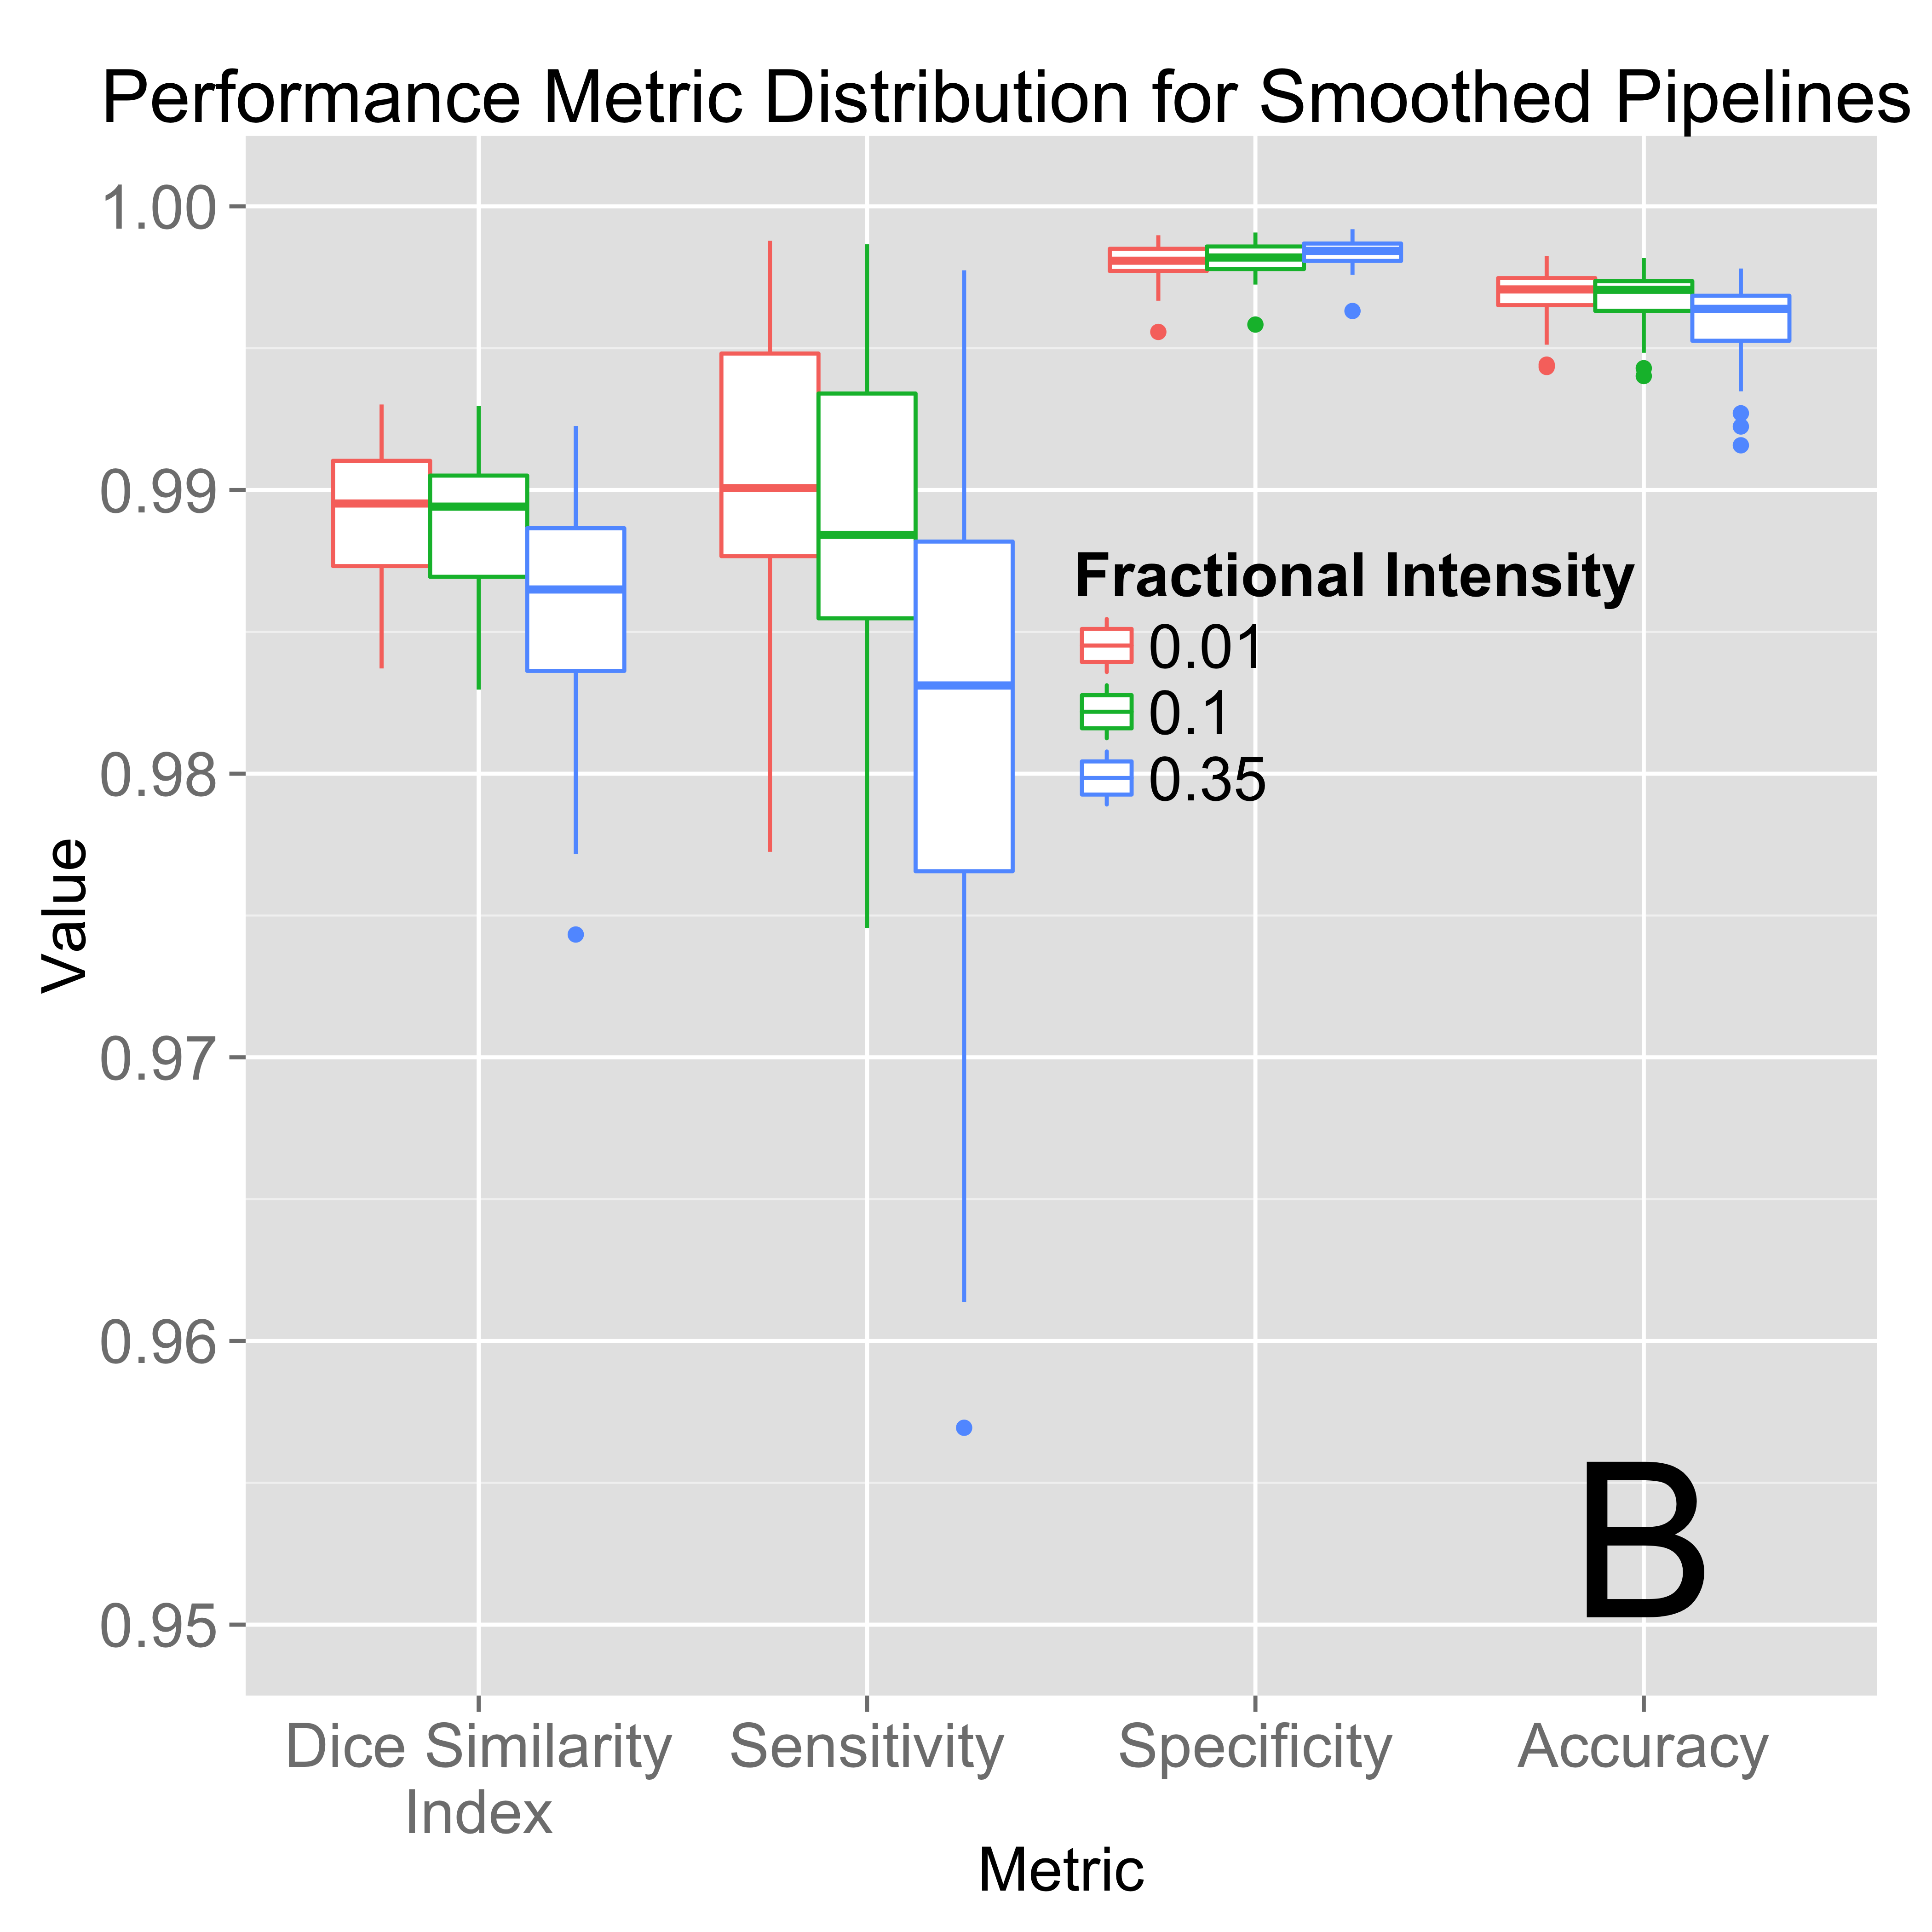
\includegraphics[width=0.46\linewidth]{figure/CT_Skull_Stripping_Figure2b.png} \\
\end{tabular}
\newline
{\bf Performance Metric Distribution for Different Pipelines.} Panel~A displays the performance for brain extraction for the pipelines, panel~B focuses on only those using smoothed images. 
Using an FI of $0.01$ or $0.1$ performed better than $0.35$.  Using an FI of $0.01$ had a higher median sensitivity ($0.9902$) than an FI of $0.1$ ($0.9891$, $p< 0.001$), lower specificity ($0.998$ vs. $0.998$; $p< 0.001$), and no difference in accuracy ($0.9971$ vs. $0.9971$; $p= 0.039$) or DSI ($0.9892$ vs. $0.9895$).



\section{Smoothing Images can Dramatically Increase Performance}

\begin{figure}[htb]
\begin{tabular}{cc}
	\includegraphics[width=0.35\linewidth]{figure/{101-307_20061110_1638_CT_5_RM_Head_SS_0.01_Mask}.png} &
	\includegraphics[width=0.35\linewidth]{figure/{101-307_20061110_1638_CT_5_RM_Head_SS_0.01_nopresmooth_Mask}.png}  
\end{tabular}
\label{fig:ss_example}
\end{figure}

\vfill

\end{minipage}
\begin{minipage}{0.39\linewidth}

%\columnbreak

%
%\begin{SCfigure}[][h]
%  \subfloat{
%  \label{unsmoothed}
%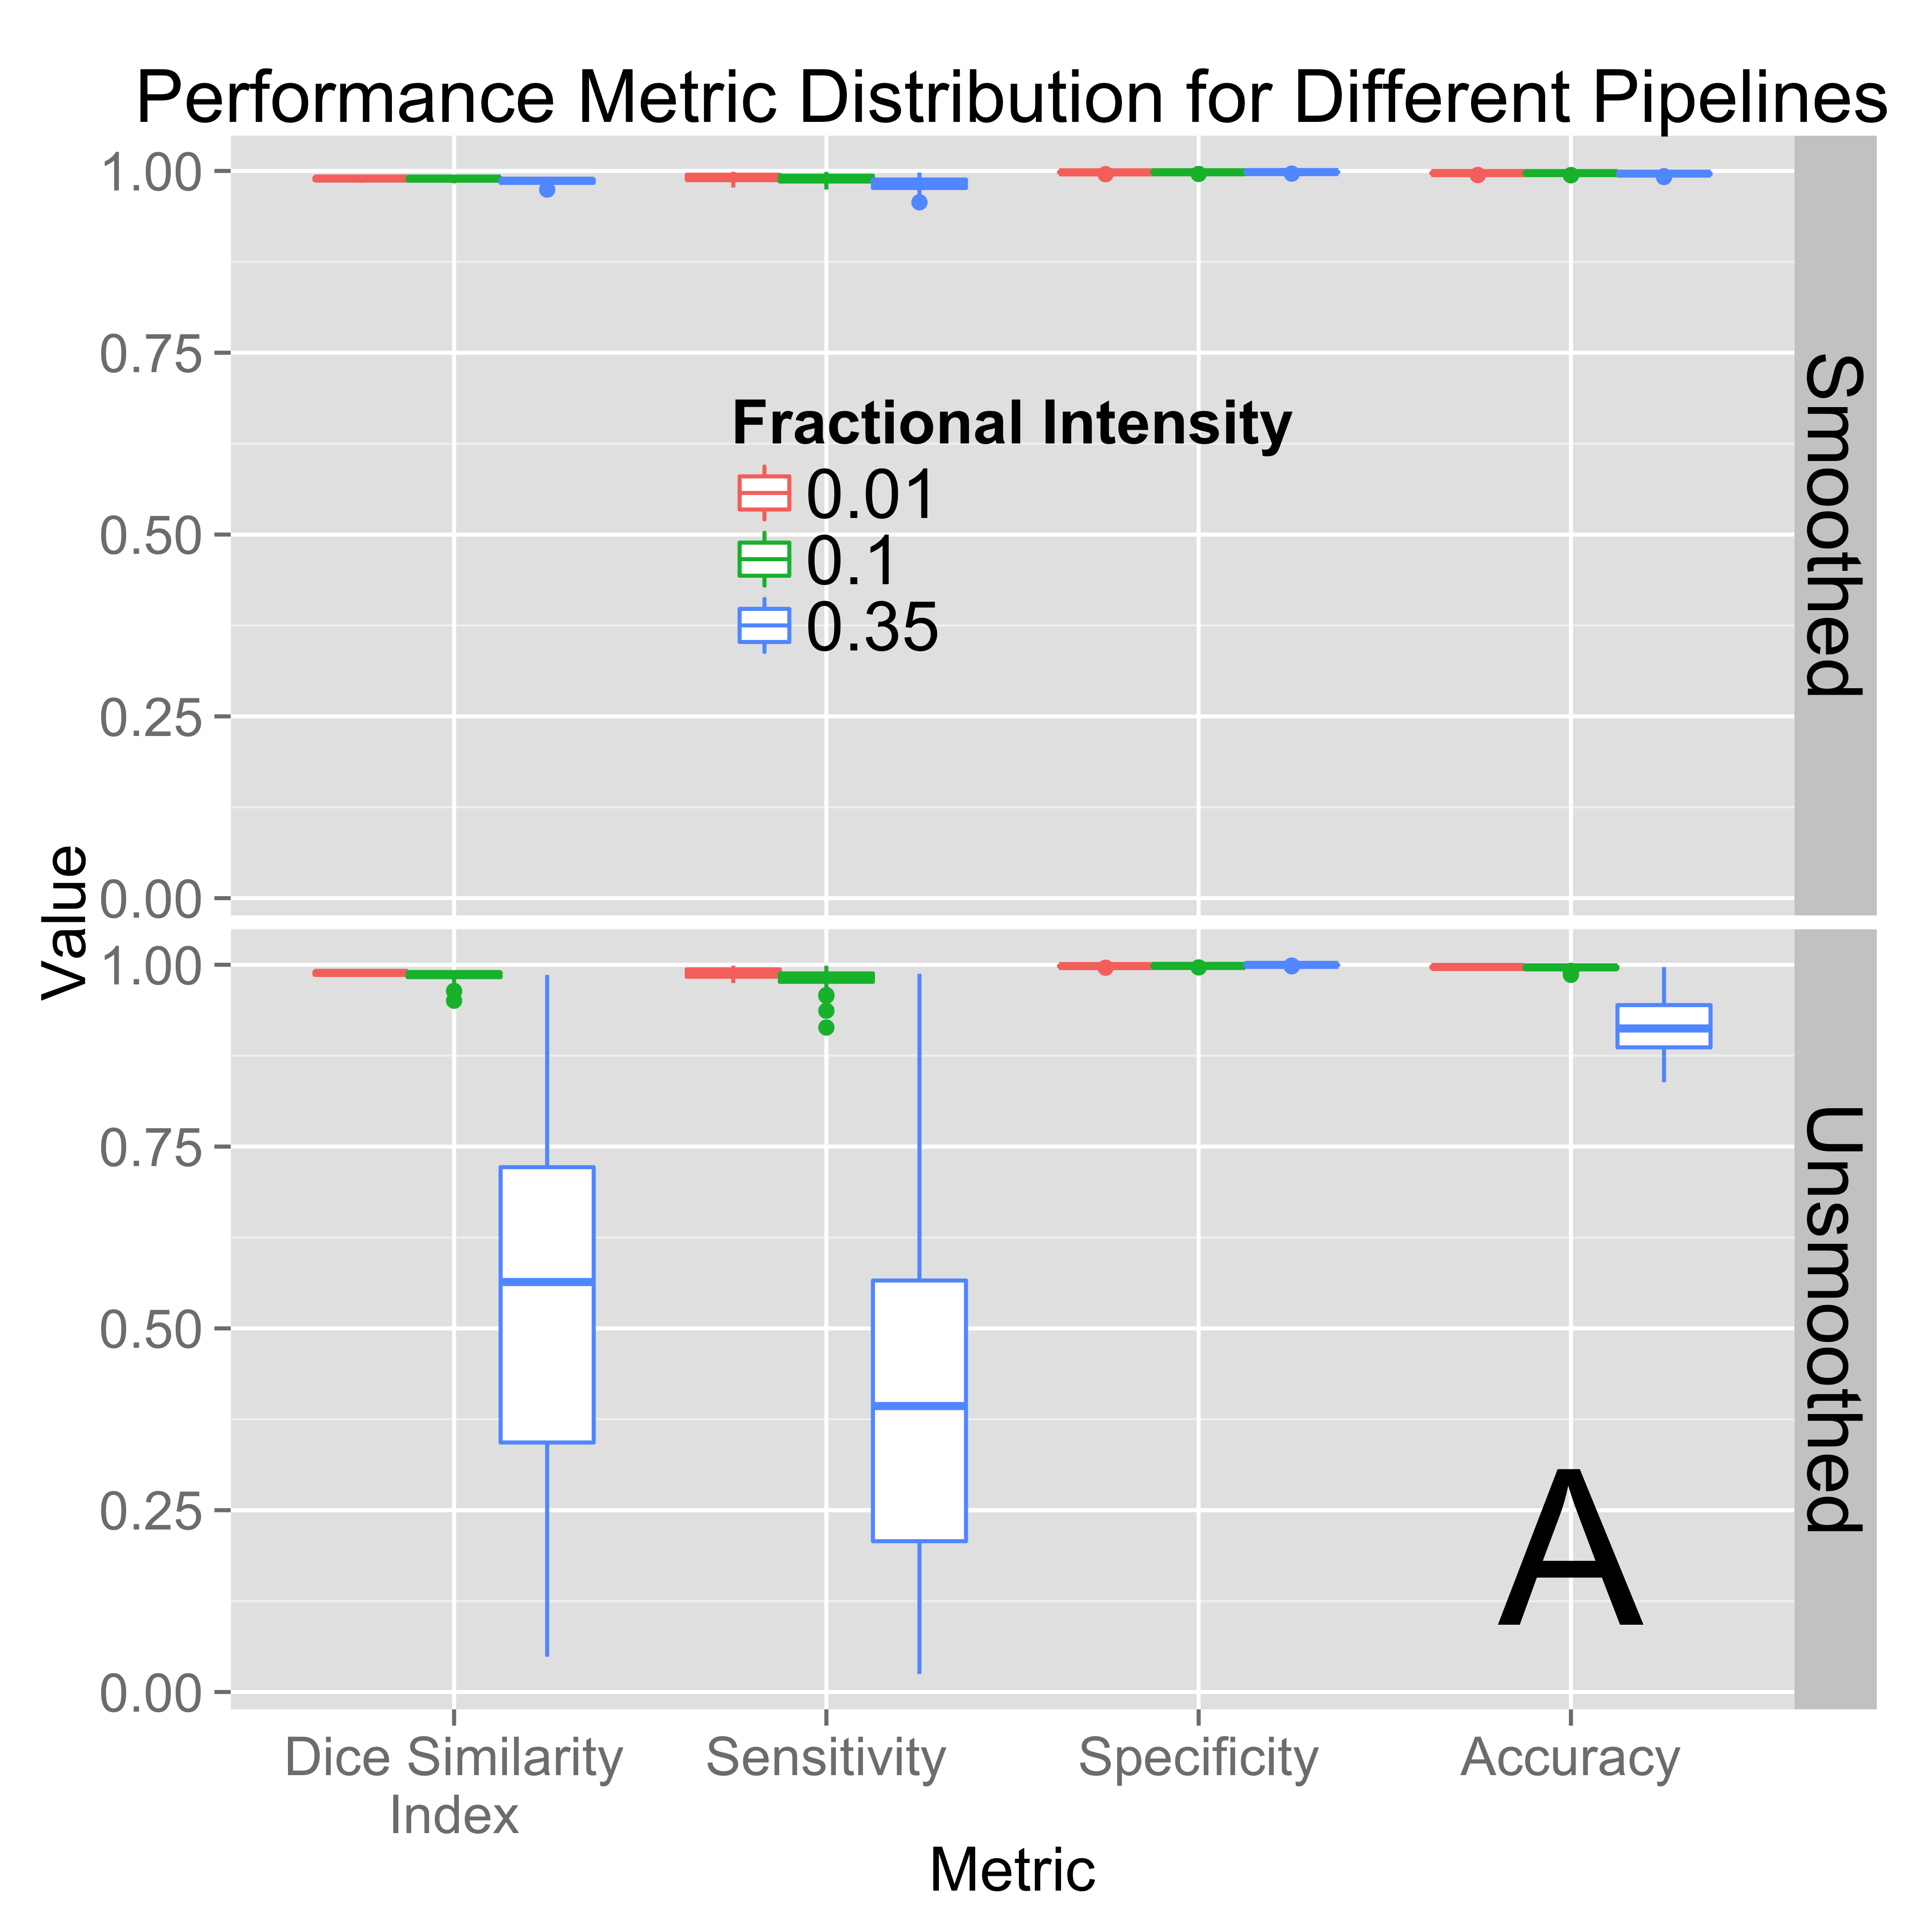
\includegraphics[width=.33\textwidth]{figure/CT_Skull_Stripping_Figure2.png}
%}
%\hfill
%  \subfloat{
%  \label{smoothed}
%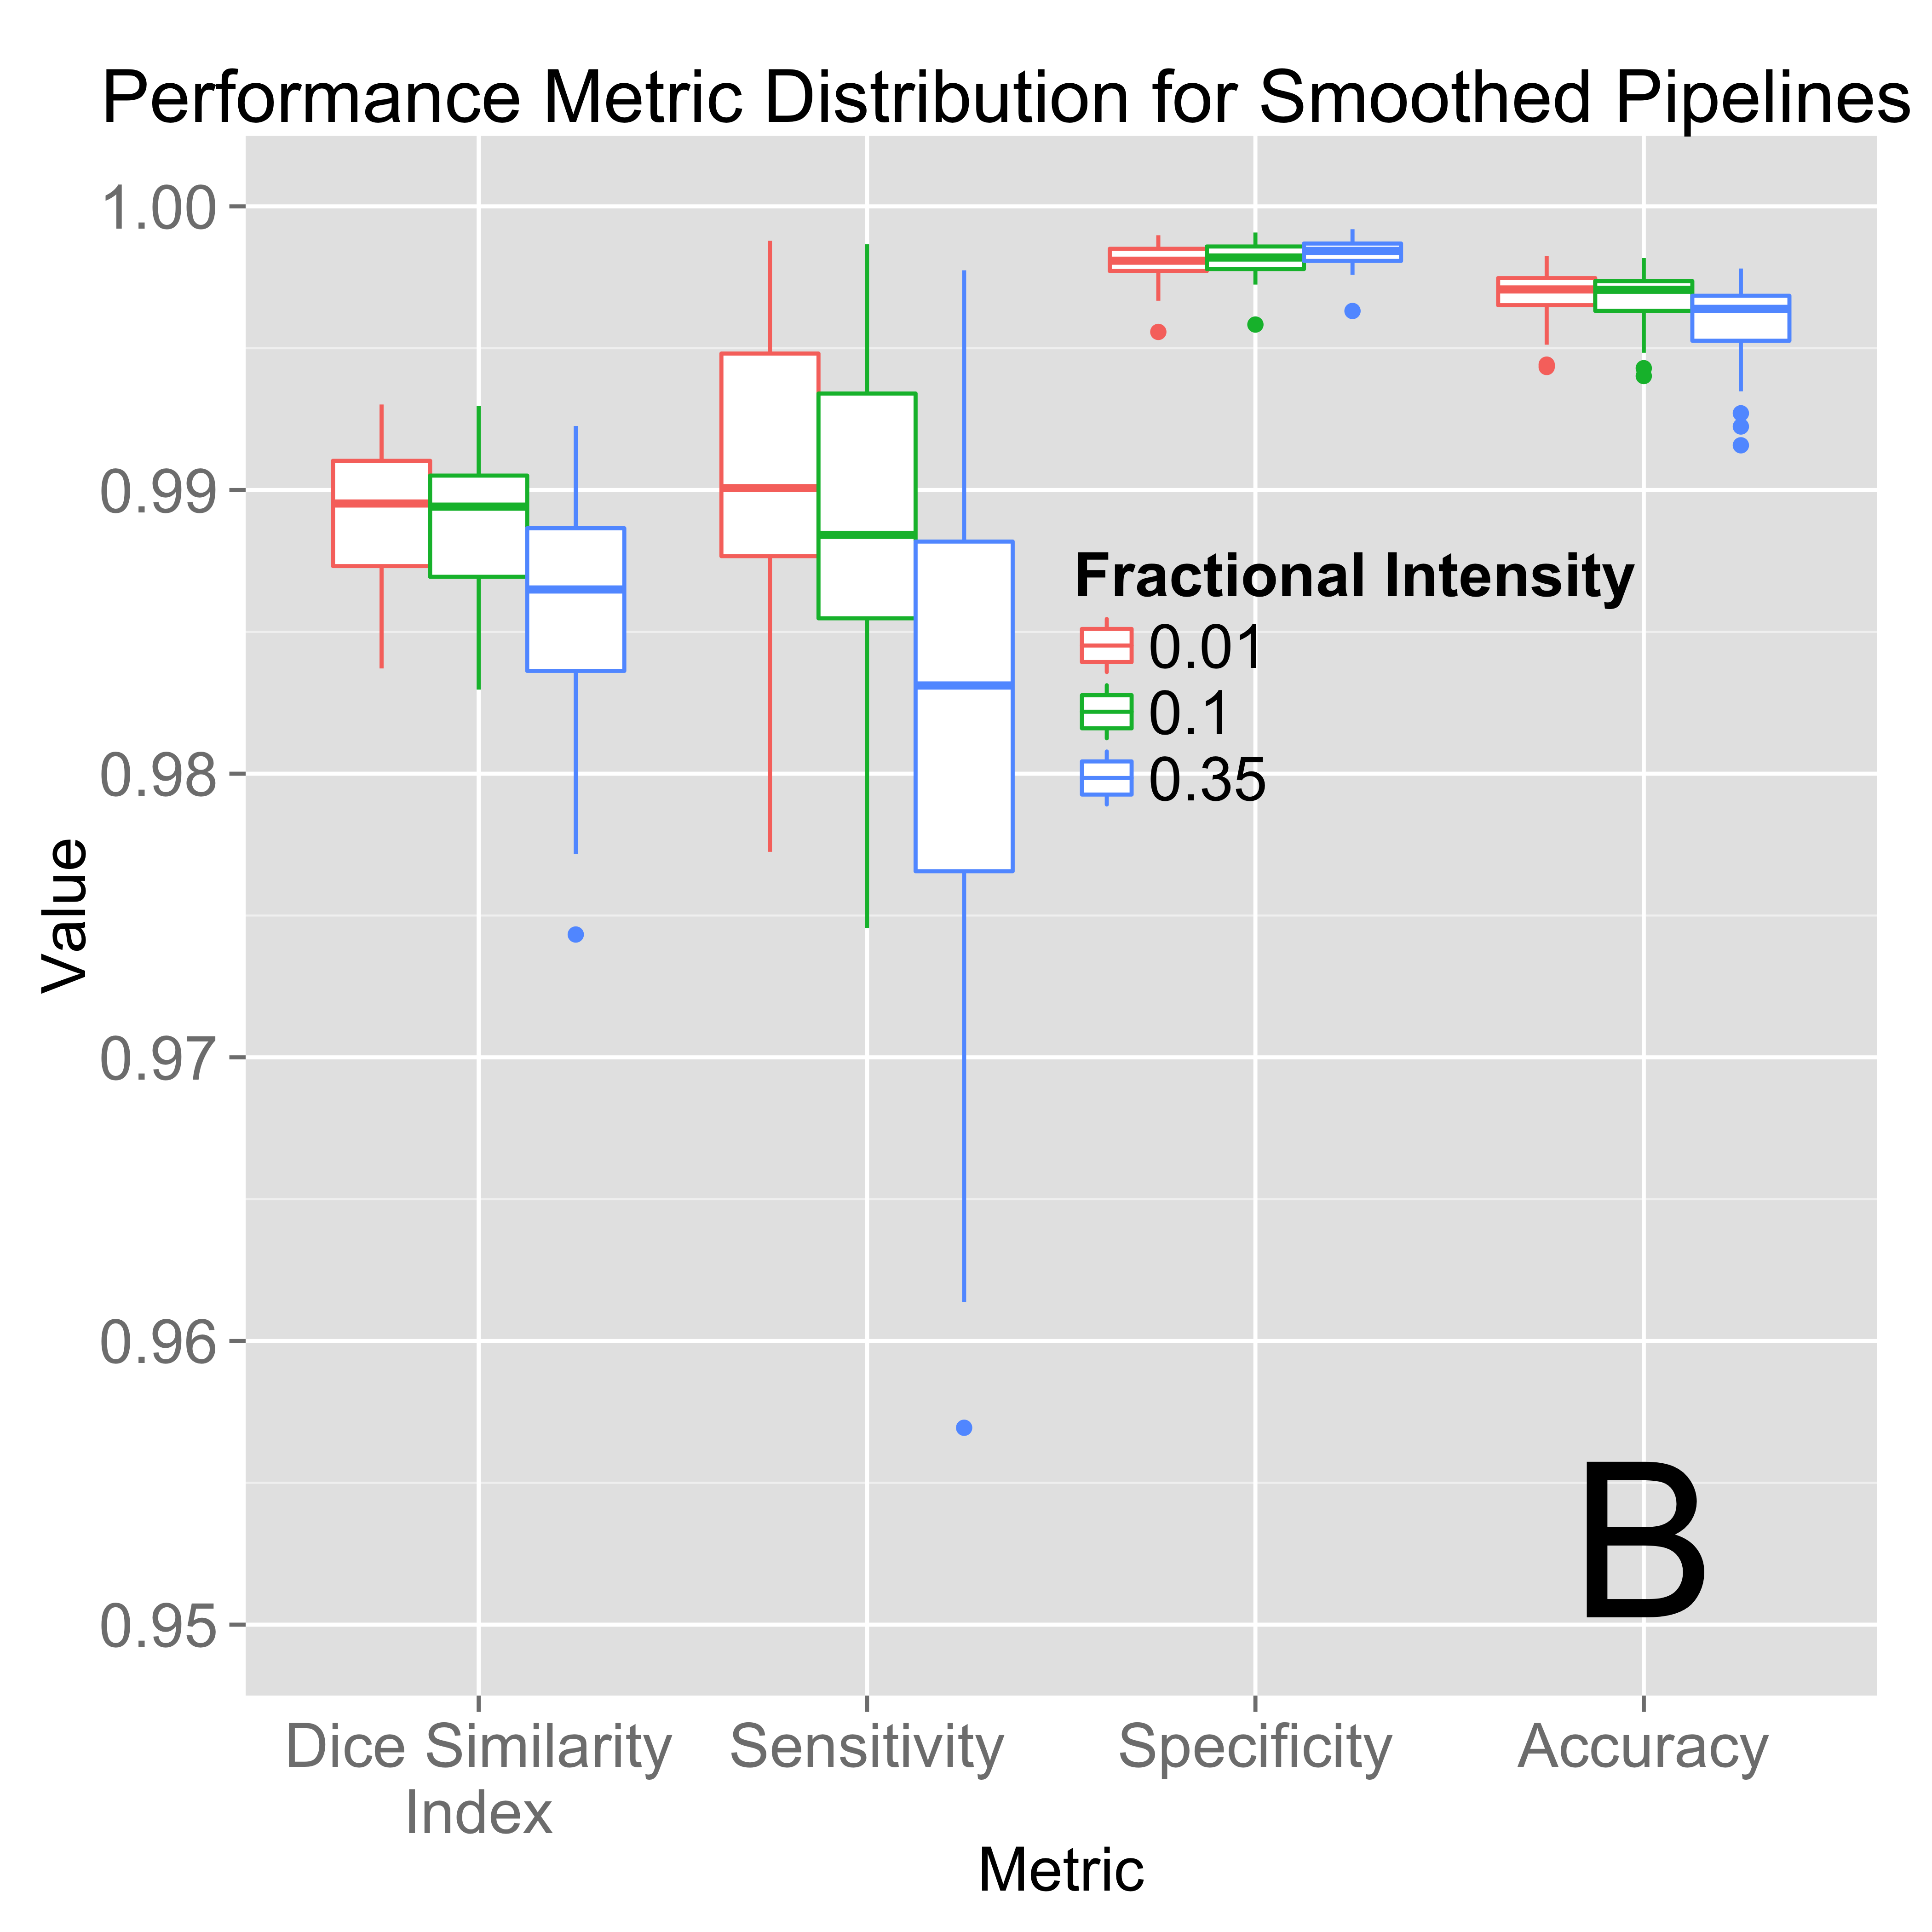
\includegraphics[width=.33\textwidth]{figure/CT_Skull_Stripping_Figure2b.png}
%}
%\caption{CT_Skull_Stripping_Figure2}
%\label{fig:metrics}
%\end{SCfigure}

\section{ CT Skull Stripping Leads to Consistent Intracranial Volume Estimates}

\begin{tabular}{cc}
	\includegraphics[width=0.45\linewidth]{../results/Intraclass_Correlation_no_crani_check_fill.png} &
	\includegraphics[width=0.45\linewidth]{../results/Intraclass_Correlation_no_crani_check_day10.png} 
\end{tabular}

{\bf Intracranial Volume (ICV) Estimate over Time.}  Each line represents an individual patient's ICV estimate over time.  The data presented used an FI $= 0.01$ and smoothed data.   The left panel shows all data used to estimate the intraclass correlation coefficient (ICC) of $0.93, (95\% CI: 0.91, 0.95)$.  

%\input{../demographics_short.tex}
%l

%--References------------------------------------------------------------------
\section{Where does it fail?}
\begin{center}
\begin{tabular}{>{\centering}m{0.25\linewidth}>{\centering}m{0.25\linewidth}>{\centering\arraybackslash}m{0.25\linewidth}}
\includegraphics[width=\linewidth]{../results/Neck_Fail.png} &
\includegraphics[width=\linewidth]{../results/Crani_Fail.png} & 
\includegraphics[width=\linewidth]{../results/Total_Fail.png} \\
Much more area than the brain is imaged &
Patient had a craniotomy & 
CT ventricles are low intensity or enlarged 
\end{tabular}
\end{center}

\section{We have code to do this!}

\begin{tabular}{m{0.5\linewidth} m{0.5\linewidth} }
$\bullet$ R code: \url{http://bit.ly/CTBET_RCODE} & $\bullet$ bash code: \url{http://bit.ly/CTBET_BASH}
\end{tabular}


\section{Conclusions}
\vspace*{-0.5cm}
Smoothing the data using a conservative smoother ($1$mm Gaussian kernel) and using an FI of $0.01$ provides good brain extraction.




%\renewcommand{\bibname}{\chapter{References}}
\section{References}
\setlength\bibitemsep{0pt}
\printbibliography[heading=none]\vspace*{-0.5cm}


%==============================================================================
%==End of content==============================================================
%==============================================================================


%--End of references-----------------------------------------------------------

%\end{multicols}
\end{minipage}
%==============================================================================
\end{frame}
\end{document}

